\subchapter{Accessing Hardware Devices}
{Objective: learn how to access hardware devices and declare new ones.}

\section{Goals}

Now that we have access to a command line shell thanks to a working root
filesystem, we can now explore existing devices and make new ones
available. In particular, we will make changes to the Device Tree
and compile an out-of-tree Linux kernel module.

\section{Setup}

Go to the \code{$HOME/__SESSION_NAME__-labs/hardware} directory,
which provides useful files for this lab.

However, we will go on booting the system through NFS, using the
root filesystem built by the previous lab.

\section{Exploring /dev}

Start by exploring \code{/dev} on your target system. Here are a few
noteworthy device files that you will see:

\begin{itemize}
 \item {\em Terminal devices}: devices starting with \code{tty}.
       Terminals are user interfaces taking text as
       input and producing text as output, and are typically used by
       interactive shells. In particular, you will find
       \code{console} which matches the device specified through
       \code{console=} in the kernel command line. You will also find
       the {\tt \ttyname} device file.
 \item {\em Pseudo-terminal devices}: devices starting with \code{pty},
       used when you connect through SSH for example. Those are virtual
       devices, but there are so many in \code{/dev} that we wanted
       to give a description here.
 \item {MMC device(s) and partitions}: devices starting with
       \code{mmcblk}. You should here recognize the MMC device(s)
       on your system and the associated partitions.
 \item If you have a real board (not QEMU) and a USB stick, you could
       plug it in and if your kernel was built with USB host and mass
       storage support, you should see a new \code{sda} device appear,
       together with the \code{sda<n>} devices for its partitions.
\end{itemize}

Don't hesitate to explore \code{/dev} on your workstation too
and ask any questions to your instructor.

\section{Exploring /sys}

The next thing you can explore is the {\em Sysfs} filesystem.

A good place to start is \code{/sys/class}, which exposes devices
classified by the kernel frameworks which manage them.

For example, go to \code{/sys/class/net}, and you will see all the
networking interfaces on your system, whether they are internal,
external or virtual ones.

Find which subdirectory corresponds to the network connection
to your host system, and then check device properties such as:
\begin{itemize}
   \item \code{speed}: will show you whether this is a gigabit
         or hundred megabit interface.
   \item \code{address}: will show the device MAC address. No
	 need to get it from a complex command!
   \item \code{statistics/rx_bytes} will show you how many bytes
	 were received on this interface.
\end{itemize}

Don't hesitate to look for further interesting properties by yourself!

You can also check whether \code{/sys/class/thermal} exists and is not
empty on your system. That's the thermal framework, and it allows
to access temperature measures from the thermal sensors on your system.

Next, you can now explore all the buses (virtual or physical) available
on your system, by checking the contents of \code{/sys/bus}.

In particular, go to \code{/sys/bus/mmc/devices} to see all the
MMC devices on your system. Go inside the directory for the first device
and check several files (for example):

\begin{itemize}
\item \code{serial}: the serial number for your device.
\item \code{preferred_erase_size}: the preferred erase block for your
      device. It's recommended that partitions start at multiples of this
      size.
\item \code{name}: the product name for your device. You could display
      it in a user interface or log file, for example.
\end{itemize}

Don't hesitate to spend more time exploring \code{/sys} on your system
and asking questions to your instructor.

\section{Driving GPIOs}

At this stage, we can only explore GPIOs through the legacy interface
in \code{/sys/class/gpio}, because the {\em libgpiod} interface
commands are provided through a dedicated project which we have to
build separately, and {\em Busybox} does not provide a
re-implementation for the {\em libgpiod} tools. In a later lab, we
will build {\em libgpiod} tools which use the modern
\code{/dev/gpiochipX} interface.

The first thing to do is to enable this legacy interface by enabling
\kconfig{CONFIG_GPIO_SYSFS} in the kernel configuration. Also make sure
{\em Debugfs} is enabled (\kconfig{CONFIG_DEBUG_FS} and
\kconfig{CONFIG_DEBUG_FS_ALLOW_ALL}).

After rebooting the new kernel, the first thing to do is to mount
the {\em Debugfs} filesystem:

\begin{bashinput}
# mount -t debugfs debugfs /sys/kernel/debug/
\end{bashinput}

Then, you can check information about available GPIOs banks and which
GPIOs are already in use:

\begin{bashinput}
# cat /sys/kernel/debug/gpio
\end{bashinput}

We are going to use one of the free GPIOs on the expansion headers of the board,
which is not already used by another device.

Take one of the M-M breadboard wires provided by your instructor and:
\begin{itemize}
  \item Connect one end to pin 12 of connector P9
  \item Connect the other end to pin 1 (\code{DGND}) of connector P9
\end{itemize}

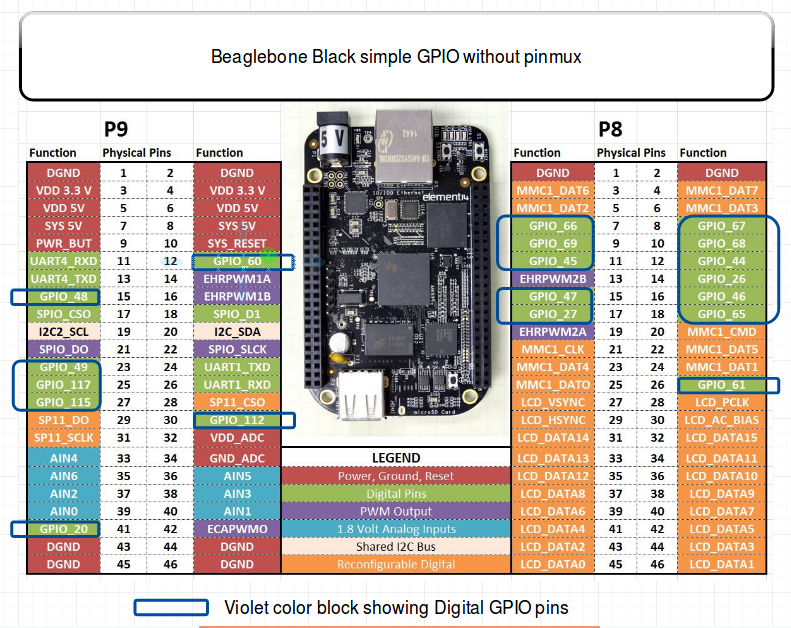
\includegraphics[width=\textwidth]{labs/sysdev-accessing-hardware-bbb/bbb-gpios.png}
{\small Source: \url{https://elinux.org/File:BBB_I-O_pins_.png}}

If you check the description of the P9 connector on the board
\href{https://github.com/beagleboard/beaglebone-black/wiki/System-Reference-Manual\#712-connector-p9}{System Reference Manual},
you can see that pin 12 is now called \code{GPIO1_28}
instead of \code{GPIO_60} in the above diagram.
This pin is already configured as a GPIO by default
(no need to change pin muxing to use this pin as a GPIO).

If you get back to the contents of \code{/sys/kernel/debug/gpio}, you'll
recognize the association between \code{gpio-28} on GPIO pin bank 0
(\code{gpiochip0}) and header pin \code{P9_12}. That's very useful
information, but you don't have this level of details for all boards,
unfortunately.

We now have everything we need to drive this GPIO using the legacy
interface. First, let's enable it:

\begin{bashinput}
# cd /sys/class/gpio
# echo %\gpionum% > export
\end{bashinput}

If indeed the pin is still available, this should create a new
{\tt gpio\gpionum} file should appear in \code{/sys/class/gpio}.

We can now configure this pin as input:

\begin{bashinput}
# echo in > gpio%\gpionum%/direction
\end{bashinput}

And check its value:

\begin{bashinput}
# cat gpio%\gpionum%/value
0
\end{bashinput}

The value should be \code{0} as the pin is connected to a ground level.

{Now, let's connect our GPIO pin to pin 3 (\code{VDD
3.3V}) of connector P9. Check the above diagram if needed.

Let's check the value again:

\begin{bashinput}
# cat gpio%\gpionum%/value
1
\end{bashinput}

The value is \code{1} because our pin is connected to a 3.3V level now.

You could use this GPIO to add a button switch to your board, for
example.

Note that you could also configure the pin as output and set its value
through the \code{value} file. This way, you could add an external LED
to your board, for example.

Before moving on to the next section, you can also check
\code{/sys/kernel/debug/gpio} again, and see that {\tt gpio-\gpionum} is now
in use, through the sysfs interface, and is configured as an input pin.

When you're done, you can see your GPIO free:

\begin{bashinput}
# echo %\gpionum% > unexport
\end{bashinput}

\section{Driving LEDs}

First, make sure your kernel is compiled with
\kconfigval{CONFIG_LEDS_CLASS}{y}, \kconfigval{CONFIG_LEDS_GPIO}{y}
and \kconfigval{CONFIG_LEDS_TRIGGER_TIMER}{y}.

Then, go to \code{/sys/class/leds} to see all the LEDs that you are allowed
to control.

Let's control the LED which is called
\code{beaglebone:green:heartbeat}.

Go into the directory for this LED, and check its trigger (what
routine is used to drive its value):

\begin{bashinput}
# cat trigger
\end{bashinput}

As you can see, there are many triggers to choose from, the current
being \code{heartbeat}, corresponding to the CPU activity.

You can disable all triggers by:

\begin{bashinput}
# echo none > trigger
\end{bashinput}

And then directly control the LED:

\begin{bashinput}
# echo 1 > brightness
# echo 0 > brightness
\end{bashinput}

You could also use the \code{timer} trigger to light the LED
with specified time on and time off:

\begin{bashinput}
# echo timer > trigger
# echo 10 > delay_on
# echo 200 > delay_off
\end{bashinput}

\section{Managing the I2C buses and devices}

\subsection{Enabling an I2C bus}

The next thing we want to do is connect an Nunchuk joystick
to an I2C bus on our board. The I2C bus is very frequently used
to connect all sorts of external devices. That's why we're covering
it here.

As shown on the below picture found on
\url{https://elinux.org/Beagleboard:Cape_Expansion_Headers}, the
BeagleBone Black has two I2C busses available on its expansion headers:
I2C1 and I2C2. Another one exists (I2C0), but it's not
available on the external headers.

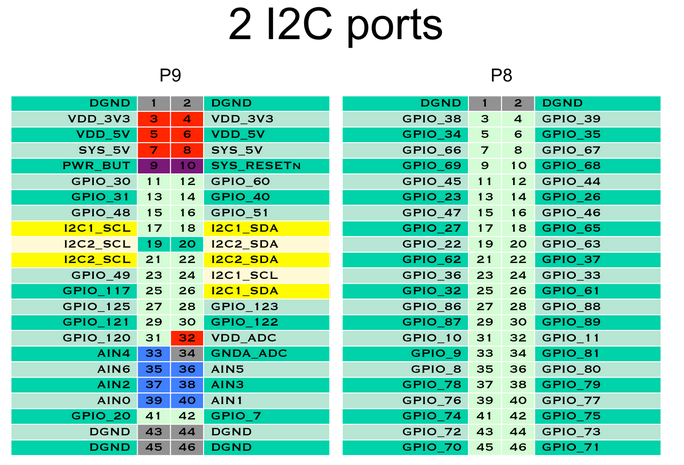
\includegraphics[width=0.7\textwidth]{labs/sysdev-accessing-hardware-bbb/bbb-i2c.png}

In this lab, we will try to use I2C1 on P9 pins 17 and 18, because it's more
interesting to use than I2C2 which is already enabled by default.

So, let's see which I2C buses are already enabled:

\begin{bashinput}
# i2cdetect -l
i2c-2	i2c             OMAP I2C adapter                        I2C adapter
i2c-0	i2c             OMAP I2C adapter                        I2C adapter
\end{bashinput}

Here you can see that I2C1 is missing.

As the bus numbering scheme in Linux doesn't always match the one
on the datasheets, let's check the base addresses of the registers
of these controllers:

\begin{bashinput}
# ls -l /sys/bus/i2c/devices/i2c-*
lrwxrwxrwx    1         0 Jan  1 00:59 /sys/bus/i2c/devices/i2c-0 -> ../../../devices/platform/ocp/44c00000.interconnect/44c00000.interconnect:segment@200000/44e0b000.target-module/44e0b000.i2c/i2c-0
lrwxrwxrwx    1         0 Jan  1 00:59 /sys/bus/i2c/devices/i2c-2 -> ../../../devices/platform/ocp/48000000.interconnect/48000000.interconnect:segment@100000/4819c000.target-module/4819c000.i2c/i2c-2
\end{bashinput}

That's not completely straighforward, but you can supposed that:
\begin{itemize}
\item I2C0 is at address \code{0x44e0b000}
\item I2C2 is at address \code{0x4819c000}
\end{itemize}

Now let's double check the addressings by looking at the
\href{https://www.ti.com/lit/ug/spruh73q/spruh73q.pdf}{TI AM335x SoC
datasheet}, in the \code{L4_WKUP Peripheral Memory Map} section:

\begin{itemize}
\item I2C0 is indeed at address \code{0x44e0b000}
\item I2C1 is at address \code{0x4802a000}
\item I2C2 is indeed at address \code{0x4819c000}
\end{itemize}

So, we are lucky that \code{i2c-0} in Linux corresponds to I2C0 in the
datasheet, and that \code{i2c-2} corresponds to I2C2.
We're just missing \code{i2c-1}.

\subsection{Customizing the Device Tree}

Fortunately, \busname\ is already defined in the one of the DTS includes
used by the Device Tree for our board. In our case, that's in
\kfile{arch/arm/boot/dts/am33xx-l4.dtsi}. Look by yourself in this
file, and you will find its definition, but with \code{status =
"disabled";}. This means that this I2C controller is not enabled yet,
and it's up to boards using it to do so.

We could modify the \kfile{arch/arm/boot/dts/am335x-boneblack.dts} file
for our board, but that's not a very good idea as this file is
maintained by the kernel developers. The changes that you make could
collide with future changes made by the maintainers for this file.

A more futureproof idea is to create a new Device Tree file which
includes the standard one, and adds custom definitions. So, create a
new \code{arch/arm/boot/dts/am335x-boneblack-custom.dts} file containing:

\begin{verbatim}
/dts-v1/;
#include "am335x-boneblack.dts"

&i2c1 {
        status = "okay";
};
\end{verbatim}

As you can see, it's also possible to include \code{dts} files, and not
only \code{dtsi} ones.

Modify the \kfile{arch/arm/boot/dts/Makefile} file to add your custom
Device Tree, and then have it compiled (\code{make dtbs}).

Reboot your board with the update.

Back to the running system, we can now see that there is one more
I2C bus:

\begin{bashinput}
# i2cdetect -l
i2c-1	i2c             OMAP I2C adapter                        I2C adapter
i2c-2	i2c             OMAP I2C adapter                        I2C adapter
i2c-0	i2c             OMAP I2C adapter                        I2C adapter
\end{bashinput}

Run the below command to confirm that the new bus has the same address
as in the datasheet (\code{0x4802a000}):

\bashcmd{ls -l /sys/bus/i2c/devices/i2c-1}

Now, let's use \code{i2cdetect}'s capability to probe a bus for devices.
Let's start by the bus associated to \code{i2c-0}:

\begin{bashinput}
# i2cdetect -r 0
i2cdetect: WARNING! This program can confuse your I2C bus
Continue? [y/N] y
     0  1  2  3  4  5  6  7  8  9  a  b  c  d  e  f
00:          -- -- -- -- -- -- -- -- -- -- -- -- --
10: -- -- -- -- -- -- -- -- -- -- -- -- -- -- -- --
20: -- -- -- -- UU -- -- -- -- -- -- -- -- -- -- --
30: -- -- -- -- 34 -- -- -- -- -- -- -- -- -- -- --
40: -- -- -- -- -- -- -- -- -- -- -- -- -- -- -- --
50: 50 -- -- -- -- -- -- -- -- -- -- -- -- -- -- --
60: -- -- -- -- -- -- -- -- -- -- -- -- -- -- -- --
70: -- -- -- -- -- -- -- --
\end{bashinput}

We can see three devices on this internal bus:
\begin{itemize}
\item One at address \code{0x24}, indicated by \code{UU},
      which means that there is a kernel driver actively
      driving this device.
\item Two other devices at addresses \code{0x34} and \code{0x50}.
      We just know that they are currently not bound to a kernel driver.
\end{itemize}

Now try to probe \busname\  through \code{i2cdetect -r 1}.

You will see that the command will fail to connect to
the bus. That's because the corresponding signals are
not exposed yet to the outside connectors through pin muxing.

So, get back to your custom Device Tree and add pin muxing definitions
for I2C1 (we took them from a device tree from another board with the same
CPU: \kfile{arch/arm/boot/dts/am335x-evm.dts}) and refer to these
definitions in the \code{i2c1} node through the \code{pinctrl-names}
and \code{pinctrl-0} properties:

\begin{verbatim}
/dts-v1/;
#include "am335x-boneblack.dts"

&am33xx_pinmux {
  i2c1_pins: pinmux_i2c1_pins {
    pinctrl-single,pins = <
      AM33XX_PADCONF(AM335X_PIN_SPI0_CS0, PIN_INPUT_PULLUP, MUX_MODE2) /* spi0_cs0.i2c1_scl */
      AM33XX_PADCONF(AM335X_PIN_SPI0_D1, PIN_INPUT_PULLUP, MUX_MODE2) /* spi0_d1.i2c1_sda */
    >;
  };
};

&i2c1 {
        pinctrl-names = "default";
        pinctrl-0 = <&i2c1_pins>;
        status = "okay";
};
\end{verbatim}

You can understand the above values thanks to the pin muxing diagram for
connector P9, available at \url{https://elinux.org/images/b/b4/HeaderP9.jpg},
which was extracted from the board System Reference Manual:

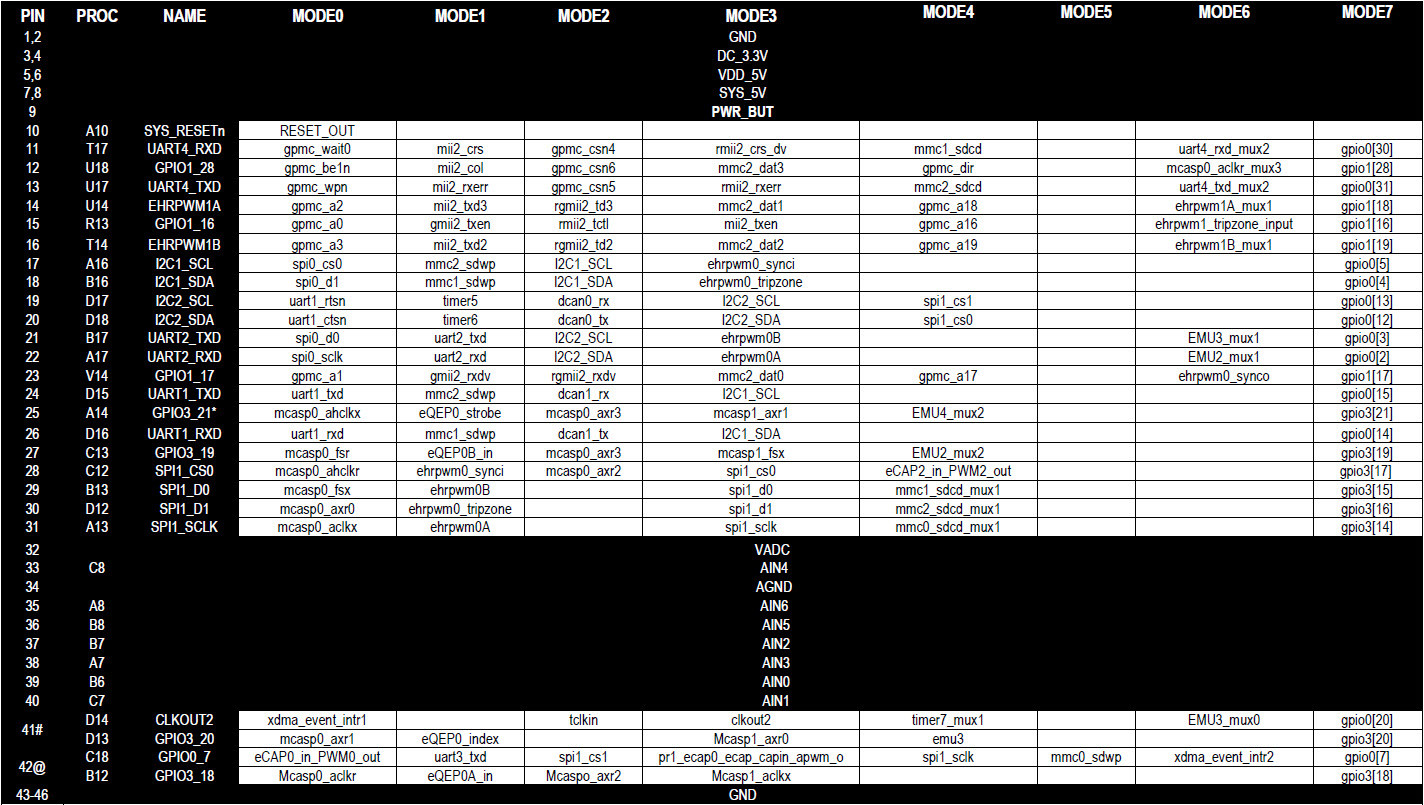
\includegraphics[width=\textwidth]{labs/sysdev-accessing-hardware-bbb/bbb-p9-pinmux.jpg}

\begin{itemize}
  \item \code{AM335X_PIN_SPI0_CS0} and \code{AM335X_PIN_SPI0_D1} are
        the offsets of the registers controlling pin muxing for the
	corresponding pins of the SoC package.
  \item \ksym{MUX_MODE2} corresponds to \code{MODE2}, to get I2C1 SCL and SDA
	signals on such pins.
  \item \ksym{PIN_INPUT_PULLUP} is one of the supported options for
        these pins.
\end{itemize}

Recompile your Device Tree and reboot.

You should now be able to probe your bus:

\begin{bashinput}
# i2cdetect -r 1
i2cdetect: WARNING! This program can confuse your I2C bus
Continue? [y/N] y
     0  1  2  3  4  5  6  7  8  9  a  b  c  d  e  f
00:          -- -- -- -- -- -- -- -- -- -- -- -- --
10: -- -- -- -- -- -- -- -- -- -- -- -- -- -- -- --
20: -- -- -- -- -- -- -- -- -- -- -- -- -- -- -- --
30: -- -- -- -- -- -- -- -- -- -- -- -- -- -- -- --
40: -- -- -- -- -- -- -- -- -- -- -- -- -- -- -- --
50: -- -- -- -- -- -- -- -- -- -- -- -- -- -- -- --
60: -- -- -- -- -- -- -- -- -- -- -- -- -- -- -- --
70: -- -- -- -- -- -- -- --
\end{bashinput}

No device is detected yet, because this bus is just
used for external devices. It's time to add one though.

\subsection{Adding and enabling an I2C device}

Let's connect the Nunchuk provided by your instructor
to the \busname\ bus on the board, using breadboard wires:

\includegraphics[width=0.3\textwidth]{common/nunchuk-pinout.pdf}
\includegraphics[width=0.7\textwidth]{common/bbb-connect-nunchuk.pdf}

\begin{itemize}
\item Connect the Nunchuk PWR pin to pin 4 (3V3) of connector P9
\item Connect the Nunchuk GND pin to pin 1 (GND) of connector P9
\item Connect the Nunchuk SCL pin to pin 17 of connector P9
\item Connect the Nunchuk SDA pin to pin 18 of connector P9
\end{itemize}

If you didn't do any mistake, your new device should be detected at
address \code{0x52}:

\begin{bashinput}
# i2cdetect -r 1
i2cdetect: WARNING! This program can confuse your I2C bus
Continue? [y/N] y
     0  1  2  3  4  5  6  7  8  9  a  b  c  d  e  f
00:          -- -- -- -- -- -- -- -- -- -- -- -- --
10: -- -- -- -- -- -- -- -- -- -- -- -- -- -- -- --
20: -- -- -- -- -- -- -- -- -- -- -- -- -- -- -- --
30: -- -- -- -- -- -- -- -- -- -- -- -- -- -- -- --
40: -- -- -- -- -- -- -- -- -- -- -- -- -- -- -- --
50: -- -- 52 -- -- -- -- -- -- -- -- -- -- -- -- --
60: -- -- -- -- -- -- -- -- -- -- -- -- -- -- -- --
70: -- -- -- -- -- -- -- --
\end{bashinput}

We will later compile an out-of-tree kernel module to support this device.

\section{Plugging a USB audio headset}

In the next labs, we are going to play audio using a USB audio headset.
Let's see whether our kernel supports such hardware by plugging the
headset provided by your instructor.

Before plugging the device, look at the output of \code{lsusb}:

\begin{bashinput}
# lsusb
Bus 001 Device 001: ID 1d6b:0002
\end{bashinput}

Now, when you plug the USB headset, a number of messages should appear
on the console, and running \code{lsusb} again should show an
additional device:

\begin{bashinput}
# lsusb
Bus 001 Device 001: ID 1d6b:0002
Bus 001 Device 004: ID 1b3f:2008
\end{bashinput}

The device of vendor ID \code{1b3f} and product ID \code{2008} has
appeared. Of course, this depends on the actual USB audio device
that you used.

The device also appears in \code{/sys/bus/usb/devices/}, in a
directory whose name depends on the topology of the USB bus. When the
device is plugged in the kernel messages show:

\begin{bashinput}
usb 1-1: new full-speed USB device number 4 using musb-hdrc
usb 1-1: New USB device found, idVendor=1b3f, idProduct=2008, bcdDevice= 1.00
usb 1-1: New USB device strings: Mfr=1, Product=2, SerialNumber=0
usb 1-1: Product: USB Audio Device
usb 1-1: Manufacturer: GeneralPlus
\end{bashinput}

So if we go in \code{/sys/bus/usb/devices/1-1}, we get the {\em
sysfs} representation of this USB device:

\begin{bashinput}
# cd /sys/bus/usb/devices/1-1
# cat idVendor
1b3f
# cat idProduct
2008
# cat busnum
1
# cat devnum
4
# cat product
USB Audio Device
\end{bashinput}

However, while the USB device is detected, we currently do not have
any driver for this device, so no actual sound card is detected.

\section{Enabling, installing and using in-tree kernel modules}

Go back to the kernel source directory.

The Linux kernel has a generic driver supporting all USB audio devices
supporting the standard USB audio class. This driver can be enabled
using the \kconfig{CONFIG_SND_USB_AUDIO} configuration option. Look
for this parameter in the kernel configuration, and you should find
that it is already enabled as a module.

So, instead of compiling the corresponding driver as a built-in, that's
a good opportunity to practice with kernel modules.

So, compile your modules:
\begin{bashinput}
make modules
\end{bashinput}

Then, following details given in the lectures, install the modules in our NFS
root filesystem (\code{$HOME/__SESSION_NAME__-labs/tinysystem/nfsroot}).

Also make sure to update the kernel image (\code{make zImage}), and reboot the
board.  Indeed, due to the changes we have made to the kernel source code,
the kernel version is now \code{5.15.<x>-dirty}, the {\em dirty}
keyword indicating that the Git working tree has uncommitted changes.
The modules are therefore installed in \code{/lib/modules/5.15.<x>-dirty/},
and the version of the running Linux kernel must match this.

After rebooting, try to load the module that we need:

\begin{bashinput}
modprobe snd-usb-audio
\end{bashinput}

By running \code{lsmod}, see all the module dependencies that
were loaded too.

You can also see that a new USB device driver in
\code{/sys/bus/usb/drivers/snd-usb-audio}. This directory shows which
USB devices are bound to this driver.

You can check that \code{/proc/asound} now exists (thanks to loading
modules for the ALSA, the Linux sound subsystem), and that one sound
card is available:

\begin{bashinput}
# cat /proc/asound/cards
 0 [Device         ]: USB-Audio - USB Audio Device
                      GeneralPlus USB Audio Device at usb-musb-hdrc.1-1, full speed
\end{bashinput}

Check also the \code{/dev/snd} directory, which should now contain
some character device files. These will be used by the user-space
libraries and applications to access the audio devices.

Modify your startup scripts so that the \code{snd-usb-audio} module
is always loaded at startup.

We cannot test the sound card yet, as we will need to build some
software first. Be patient, this is coming soon.

\section{Compiling and installing an out-of-tree kernel module}

The next device we want to support is the I2C Nunchuk. There is a driver
in the kernel to support it when connected to a Wiimote controller, but
there is no such driver to support it as an I2C device.

Fortunately, one is provided in
\code{$HOME/__SESSION_NAME__-labs/hardware/data/nunchuk/nunchuk.c}. You can check
\href{https://bootlin.com/training/kernel/}{Bootlin's Linux kernel and
driver development course} to learn how to implement all sorts of device
drivers for Linux.

Go to this directory, and compile the out-of-tree module as follows:

\begin{bashinput}
make -C $HOME/__SESSION_NAME__-labs/kernel/linux M=$PWD
\end{bashinput}

Here are a few explanations:
\begin{itemize}
\item The \code{-C} option lets \code{make} know which Makefile to
      use, here the toplevel Makefile in the kernel sources.
\item \code{M=$PWD} tells the kernel Makefile to build external
      module(s) from the file(s) in the current directory.
\end{itemize}

Now, you can install the compiled module in the NFS root filesystem
by passing the \code{modules_install} target and specifying the
target directory through the \code{INSTALL_MOD_PATH} variable:

\begin{bashinput}
make -C $HOME/__SESSION_NAME__-labs/kernel/linux \
     M=$PWD \
     INSTALL_MOD_PATH=$HOME/__SESSION_NAME__-labs/tinysystem/nfsroot \
     modules_install
\end{bashinput}

You can see that this installs out-of-tree kernel modules under
\code{lib/modules/<version>/extra/}.

Back on the target, you can now check that your custom module can
be loaded:

\begin{bashinput}
# modprobe nunchuk
[ 4317.737978] nunchuk: loading out-of-tree module taints kernel.
\end{bashinput}

See \kdochtml{kbuild/modules} in kernel documentation
for details about building out-of-tree kernel modules.

However, run \code{i2cdetect -r 1} again. You will see that the
Nunchuk is still detected, but still not driven by the kernel.
Otherwise, it would be signaled by the \code{UU} character. You
may also look at the \code{nunchuk.c} file and notice a
\code{Nunchuk device probed successfully} message that you didn't
see when loading the module.

That's because the Linux kernel doesn't know about the Nunchuk
device yet, even though the driver for this kind of devices is
already loaded. Our device also has to be described in the Device Tree.

You can confirm this by having a look at the contents of the
\code{/sys/bus/i2c} directory.  It contains two subdirectories:
\code{devices} and \code{drivers}.

In \code{drivers}, there should be a \code{nunchuk} subdirectory,
but no symbolic link to a device yet. In \code{devices} you should
see some devices, but not the Nunchuk one yet.

\section{Declaring an I2C device}

To allow the kernel to manage our Nunchuk device, let's declare the
device in the custom Device Tree for our board. The declaration of the \busname\ 
bus will then look as follows:

\begin{verbatim}
&i2c1 {
        status = "okay";
        clock-frequency = <100000>;

        nunchuk: joystick@52 {
                compatible = "nintendo,nunchuk";
                reg = <0x52>;
        };
};
\end{verbatim}

Here are a few notes:
\begin{itemize}
\item The \code{clock-frequency} property is used to configure the bus
      to operate at 100 KHz. This is supposed to be required for the
      Nunchuk.
\item The Nunchuk device is added through a child node in the I2C
      controller node.
\item For the kernel to {\em probe} and drive our device, it's required
      that the \code{compatible} string matches one of the
      \code{compatible} strings supported by the driver.
\item The \code{reg} property is the address of the device on the
      I2C bus. If it doesn't match, the driver will probe the device
      but won't be able to communicate with it.
\end{itemize}

Recompile your Device Tree and reboot your kernel with the new binary.

You can now load your module again, and this time, you should see that
the Nunchuk driver probed the Nunchuk device:

\begin{bashinput}
# modprobe nunchuk
[   66.680455] nunchuk: loading out-of-tree module taints kernel.
[   66.687645] input: Wii Nunchuk as /devices/platform/ocp/48000000.interconnect/48000000.interconnect:segment@0/4802a000.target-module/4802a000.i2c/i2c-1/1-0052/input/input0
[   66.695421] Nunchuk device probed successfully
\end{bashinput}

List the contents of \code{/sys/bus/i2c/drivers/nunchuk} once again. You
should now see a symbolic link corresponding to our new device.

Also list \code{/sys/bus/i2c/devices/} again. You should now see the
Nunchuk device, which can be recognized through its \code{0052} address.
Follow the link and you should see a symbolic link back to the Nunchuk
driver!

We are not ready to use this input device yet, but at least we can test
that we get bytes when buttons or the joypad are used. In the below
command, use the same number as in the message you got in the console
(\code{event0} for \code{input0} for example):

\begin{bashinput}
# od -x /dev/input/event0
\end{bashinput}

We will use the Nunchuk to control audio playback in an upcoming lab.

\section{Setting the board's model name}

Modify the custom Device Tree file one last time to override the model
name for your system. Set the \code{model} property to
\code{BeagleBone Black media player}. Don't hesitate to ask your
instructor if you're not sure how.

Recompile the device tree, and reboot the board with it. You should see
the new model name in two different places:

\begin{itemize}
\item In the first kernel messages on the serial console.
\item In \code{/sys/firmware/devicetree/base/model}. This can be
      handy for a distribution to identify the device it's running on.
      By the way, you can explore \code{/sys/firmware/devicetree} and
      find that every subdirectory corresponds to a DT node, and every
      file corresponds to a DT property.
\end{itemize}

\section{Committing kernel tree changes}

Now that our changes to the kernel sources are over,
create a branch for your changes and create a patch for them.
{\bf Please don't skip this step} as we need it for the next labs.

First, if not done yet, you should set your identity
and e-mail address in git:

\begin{bashinput}
git config --global user.email "linus@bootlin.com"
git config --global user.name "Linus Torvalds"
\end{bashinput}

This is necessary to create a commit with the \code{git commit -s}
command, as required by the Linux kernel contribution guidelines.

Let's create the branch and the patch now:

\begin{bashinput}
git checkout -b bootlin-labs
git add arch/arm/boot/dts/am335x-boneblack-custom.dts
git commit -as -m "Custom DTS for Bootlin lab"
\end{bashinput}

We can now create the patch:\\
\texttt{git format-patch stable/linux-\workingkernel.y}

This should generate a \code{0001-Custom-DTS-for-Bootlin-lab.patch}
file.

Creating the branch will impact the versions of the kernel and the modules.
Compile your kernel and install your modules again (not necessary for the
Nunchuk one for the moment) and see the version changes through the
new based directory for modules.

Don't forget to update the kernel your board boots.

That's all for now!
